\section{Diseño de la evaluación}
\label{sec:eval-design}

El objetivo de esta evaluación es validar, en condiciones controladas y reproducibles, la eficacia del sistema propuesto para \textit{detectar} \textit{data drift} y \textit{recuperar} desempeño mediante reentrenamiento automatizado, con métricas medibles y trazables en MLflow/Prometheus \citep{Gama2014,Breck2019,Chawla2021}.

% (Bloque duplicado eliminado para evitar similitud excesiva)

\subsection{Preguntas de investigación e hipótesis}
\label{subsec:eval-rq}

El proceso de evaluación se orienta por tres preguntas de investigación que permiten verificar de manera empírica la eficacia del sistema propuesto frente a sus objetivos operativos: detección oportuna del \textit{data drift}, recuperación del desempeño del modelo y estabilidad del proceso de reentrenamiento. Cada pregunta se asocia con una hipótesis comprobable, formulada en términos cuantitativos y verificables mediante los experimentos E1 (sin \textit{drift}) y E2 (con \textit{drift} inducido).

\paragraph{RQ1 — Detección.}
Se busca determinar si el sistema de monitoreo identifica oportunamente la presencia de \textit{data drift} sin generar falsos positivos en condiciones estables.  
\textbf{Hipótesis H1:} En el escenario E1 (sin \textit{drift}), la tasa de alertas generadas es inferior al 1\,\%, mientras que en el escenario E2 (con \textit{drift}), la latencia promedio de detección (\textbf{TTFD}) no supera los 60\,s.

\paragraph{RQ2 — Recuperación del desempeño.}
Evalúa la capacidad del mecanismo de reentrenamiento automático para restablecer la calidad predictiva del modelo degradado por \textit{drift}.  
\textbf{Hipótesis H2:} En el escenario E2, los valores de F1-score y AUC obtenidos tras el reentrenamiento no son estadísticamente inferiores (diferencia $<2$ puntos porcentuales) a los de la línea base del escenario E1, cumpliendo una prueba de no–inferioridad.

\paragraph{RQ3 — Estabilidad operativa.}
Examina si la política de activación basada en \textit{edge-triggered} y \textit{cooldown} mantiene estabilidad en la operación continua, evitando ciclos repetidos de reentrenamiento (\textit{flapping}) bajo condiciones de \textit{drift} sostenido.  
\textbf{Hipótesis H3:} El número de reentrenamientos automáticos registrados no excede una activación por hora, bajo las configuraciones establecidas en los parámetros \texttt{DRIFT\_COOLDOWN\_SECONDS} y \texttt{DRIFT\_CLEAR\_STREAK}.


\subsection{Escenarios de evaluación}
\label{subsec:eval-scenarios}

\subsection{Pruebas estadísticas y p-valores}
\label{subsec:eval-tests}
Para contrastar las hipótesis y diferencias entre condiciones se emplean pruebas \textbf{no paramétricas} (Mann–Whitney U) por pares de escenarios, dada la posible no-normalidad y tamaños de muestra moderados. Se evalúan F1 y PSI como métricas principales, y las latencias \textit{TTFD}/\textit{TTR}. Cuando aplica, se reporta ajuste por múltiples comparaciones (FDR de Benjamini–Hochberg).

\begin{table}[htbp]
\centering
\caption{Pruebas de Mann–Whitney sobre F1 (job de evaluación: fase previa vs fase con \textit{drift}).}
\label{tab:mw-tests}
\begin{tabular}{lccc}
\toprule
\textbf{Fuente} & $\boldsymbol{n_{\text{pre}}}$ vs. $\boldsymbol{n_{\text{drift}}}$ & $\boldsymbol{p}$-valor & $\boldsymbol{|\delta|}$ (Cliff) \\
\midrule
Job de evaluación (\texttt{metrics\_test/eval\_training\_log.csv}) & $16$ vs. $24$ & $2.55\times10^{-3}$ & $0.57$ (grande) \\
Drift-watcher (\texttt{metrics\_test/watcher\_training\_log.csv}) & $16$ vs. $22$ & $5.07\times10^{-3}$ & $0.54$ (grande) \\
\bottomrule
\end{tabular}
\\[2pt]
\footnotesize Los tamaños de efecto siguen la regla de Cliff: $|\delta|<0.147$ (trivial), $<0.33$ (pequeño), $<0.474$ (mediano), $\ge 0.474$ (grande). El ajuste FDR coincide con los valores reportados.
\end{table}


Para garantizar la validez interna y externa de la evaluación, se definieron dos escenarios experimentales controlados y reproducibles que permiten analizar el comportamiento del sistema tanto en condiciones de estabilidad como ante desviaciones significativas en la distribución de los datos. Ambos escenarios se ejecutaron sobre el mismo entorno de infraestructura descrito en el Capítulo~\ref{sec:oe1}, utilizando \texttt{Docker~Compose} y las configuraciones base del proyecto \texttt{Arlequín}.

\paragraph{Escenario E1 — Sin \textit{drift} (condición de control).}
En este escenario, el generador de datos sintéticos mantiene inalteradas las distribuciones originales de las variables de entrada. El objetivo es establecer una línea base de comportamiento, validando que el sistema de monitoreo preserve la estabilidad del modelo y no genere alertas espurias. Este escenario permite estimar la tasa de falsos positivos de detección y comprobar la robustez del sistema ante fluctuaciones menores propias del muestreo aleatorio.

\paragraph{Escenario E2 — Con \textit{drift} inducido.}
En este caso se activa el parámetro \texttt{drift\_factor} dentro del módulo \texttt{generate\_data\_session.py}, que introduce alteraciones controladas en variables numéricas y categóricas: incrementos progresivos en \texttt{amount\_usd} y \texttt{risk\_score}, y redistribución de proporciones en \texttt{account\_type}. Dichas modificaciones se enfocan principalmente en \textbf{\textit{covariate drift}} (cambios en la distribución de las variables independientes); la afectación del \texttt{risk\_score} representa sólo una aproximación parcial al \textit{concept drift} \citep{Lu2019,Sethi2017}. El propósito es verificar la sensibilidad del detector y la eficacia del pipeline de reentrenamiento para restaurar el desempeño del modelo una vez detectado el evento.

\paragraph{Justificación de las pruebas estadísticas.}
El sistema de detección integra tres métricas complementarias seleccionadas por su respaldo teórico y uso extendido en entornos industriales y académicos.  

\begin{itemize}
    \item \textbf{Kolmogorov–Smirnov (KS):} prueba no paramétrica adecuada para detectar diferencias en la forma, media y varianza de variables continuas. Su sensibilidad a cambios sutiles en la distribución la convierte en un método estándar para evaluar \textit{drift} univariado en datos financieros o de riesgo \citep{Lu2019,Chawla2021}.
    \item \textbf{Chi–cuadrado ($\chi^2$):} medida estadística robusta para comparar frecuencias categóricas observadas y esperadas, permitiendo identificar desplazamientos en proporciones de clases o categorías \citep{Sethi2017}. Es particularmente útil en dominios donde el \textit{drift} se manifiesta en la composición de segmentos poblacionales.
    \item \textbf{Population Stability Index (PSI):} indicador agregado que resume el grado de desviación entre dos distribuciones, ampliamente utilizado en la industria para evaluar la estabilidad de modelos en producción \citep{Breck2019}. Su interpretación operativa —valores superiores a 0.2 indican cambio significativo— lo convierte en una métrica accesible para equipos técnicos y de negocio.
\end{itemize}

Estas métricas fueron seleccionadas por su \textbf{complementariedad metodológica}. Mientras KS y $\chi^2$ proporcionan sensibilidad estadística específica para distintos tipos de variables (numéricas y categóricas), el PSI actúa como un agregador global que facilita la interpretación operacional del grado de cambio. En conjunto, este enfoque híbrido equilibra el rigor estadístico con la aplicabilidad práctica, alineándose con las recomendaciones contemporáneas para la detección automática de \textit{data drift} en sistemas MLOps \citep{Gama2014,Zliobaite2016,DeSousa2023}.


\subsection{Diseño experimental}
\label{subsec:eval-design-formal}

El detalle exhaustivo de escenarios y variables se estableció en el Objetivo Específico~3 (\autoref{subsec:oe3-design}); en este capítulo se retoma únicamente la fracción necesaria para interpretar los resultados. El experimento mantiene un diseño bifactorial controlado con réplicas independientes, orientado a medir desempeño, latencia y estabilidad del pipeline ante \textit{data drift}.

\paragraph{Factores y escenarios.}
\begin{itemize}\setlength\itemsep{2pt}
  \item \textbf{Factor 1 — Condición de distribución:} \textit{E1} (flujo estacionario) frente a \textit{E2} (drift inducido). Esta definición es la misma descrita en Cap.~3 y sólo se reitera su efecto como tratamiento.
  \item \textbf{Factor 2 — Etapa del modelo en E2:} métricas \textit{pre} vs. \textit{post} reentrenamiento, registradas por el mismo job de Jenkins (evaluación) y por el drift-watcher tras disparar la acción correctiva.
\end{itemize}

\paragraph{Protocolo y replicación.}
Cada ejecución completa de los jobs se considera una réplica independiente; se realizaron $n=5$ repeticiones por condición reiniciando contenedores y reutilizando el mismo modelo inicial para asegurar comparabilidad. Cada réplica genera entre 14 y 20 ciclos de monitoreo con \texttt{SAMPLE\_MAX}=$1000$ y \texttt{LOOP\_SECONDS}=$30$. Se mantienen las salvaguardas descritas en OE3: umbrales $\alpha=0.01$ y $\tau_{\text{PSI}}=0.2$, regla de disparo $p<\alpha \lor \text{PSI}>\tau$, y mecanismos anti-\textit{flapping} (\texttt{TRIGGER\_EDGE\_ONLY}, \texttt{DRIFT\_COOLDOWN\_SECONDS}, \texttt{DRIFT\_CLEAR\_STREAK}). Las semillas determinísticas (\texttt{seed}=42,7) y la alternancia del orden E1/E2 mitigan efectos de calentamiento.

\paragraph{Hipótesis formales.}
\[
\begin{aligned}
&\textbf{H}_{0}^{(1)}: \pi_{\mathrm{alert}}^{(E1)} \ge 0.01 
&&\text{vs.}\quad \textbf{H}_{1}^{(1)}: \pi_{\mathrm{alert}}^{(E1)} < 0.01 \\[3pt]
&\textbf{H}_{0}^{(2)}: \mathbb{E}[F1_{\mathrm{post}} - F1_{\mathrm{base}}] \le -0.02 
&&\text{vs.}\quad \textbf{H}_{1}^{(2)}: \mathbb{E}[F1_{\mathrm{post}} - F1_{\mathrm{base}}] > -0.02 \\[3pt]
&\textbf{H}_{0}^{(3)}: \mathrm{TTFD} \ge 60\,\mathrm{s} \ \text{ó}\  \mathrm{TTR} \ge 300\,\mathrm{s} 
&&\text{vs.}\quad \textbf{H}_{1}^{(3)}: \mathrm{TTFD} < 60\,\mathrm{s} \ \text{y}\  \mathrm{TTR} < 300\,\mathrm{s}
\end{aligned}
\]
Las tres hipótesis corresponden, respectivamente, a RQ1–RQ3:
detección oportuna, recuperación del desempeño y estabilidad operativa.

\paragraph{Métricas y agregación.}
Las métricas instrumentadas (F1, AUC, Precisión, Recall, PSI, $p_{\min}$, TTFD, TTR, FPR y \texttt{drift\_factor}) son las mismas descritas en OE3; en esta etapa se emplean para contrastar hipótesis y cuantificar la eficiencia del pipeline. Los resultados por réplica se agregan mediante promedios e intervalos de confianza al 95\,\% calculados por \textit{bootstrap} ($B=1000$).  
Para RQ2 se aplica una prueba de no–inferioridad ($\delta=0.02$) y para RQ1 una prueba unilateral de proporciones con intervalo de Wilson.  
Las medidas de tamaño del efecto (Cohen’s~$d$ y Cliff’s~$\delta$) complementan la significancia estadística, aportando evidencia práctica del impacto del reentrenamiento y de las diferencias entre condiciones.


\subsection{Ablaciones y análisis de sensibilidad}
\label{subsec:eval-ablation}

Con el fin de evaluar la contribución individual de cada componente del detector y la estabilidad del sistema frente a variaciones paramétricas, se realizaron estudios de \textbf{ablación} y \textbf{sensibilidad}.  
Las ablaciones permiten aislar el efecto de cada módulo estadístico (PSI y $\chi^2$), mientras que las pruebas de sensibilidad exploran la respuesta del sistema ante cambios en las ventanas de muestreo y en los umbrales de decisión.  
Cada experimento se repitió cinco veces y se compararon los resultados en términos de \textbf{TTFD} (tiempo de detección), \textbf{tasa de falsos negativos} y \textbf{estabilidad operativa}.

\paragraph{Ablaciones.}
\begin{enumerate}
  \item \textbf{Ablación–PSI:} se desactiva el componente del \textit{Population Stability Index} manteniendo las pruebas KS y $\chi^2$ activas.  
  Este ensayo evalúa la contribución específica del PSI a la detección de \textit{drift} numérico, midiendo la variación $\Delta \text{TTFD}$ y el incremento en la tasa de falsos negativos. Se espera un aumento significativo en el tiempo medio de detección, dado que el PSI ofrece mayor sensibilidad a desplazamientos graduales en las distribuciones continuas \citep{Sethi2017,Lu2019}.
  
  \item \textbf{Ablación–$\chi^2$:} se deshabilita la prueba de independencia para variables categóricas, con el fin de medir la pérdida de sensibilidad frente a alteraciones en \texttt{account\_type}.  
  El objetivo es cuantificar la dependencia del sistema respecto a la detección de \textit{concept drift} categórico, especialmente en escenarios donde las proporciones de clases varían lentamente.
\end{enumerate}

\paragraph{Líneas de sensibilidad.}
\begin{enumerate}
  \item \textbf{Sensibilidad a tamaño de ventana:} se varían los parámetros \texttt{SAMPLE\_MAX} y \texttt{LOOP\_SECONDS} en \{15, 30, 60\} segundos.  
  Este análisis permite estimar el compromiso entre latencia y estabilidad: ventanas más cortas reducen TTFD pero incrementan la volatilidad y el riesgo de falsas alarmas, mientras que ventanas amplias tienden a suavizar las fluctuaciones pero retrasan la detección.

  \item \textbf{Sensibilidad a umbrales estadísticos:} se realiza un barrido sistemático sobre los valores $\alpha \in \{0.05,\,0.01,\,0.001\}$ y $\tau \in \{0.1,\,0.2,\,0.3\}$.  
  Se evalúa el impacto sobre TTFD, tasa de falsos positivos y métrica F1 post–reentrenamiento.  
  Estos experimentos permiten identificar el punto de operación óptimo entre sensibilidad y estabilidad, configurando un equilibrio adecuado para los SLO-1 y SLO-3 definidos en la sección~\ref{subsec:eval-metrics}.
\end{enumerate}

\begin{figure}[htbp]
\centering
\begin{subfigure}[b]{0.48\textwidth}
\centering
\begin{tikzpicture}
\begin{axis}[
    width=\linewidth, height=4.6cm,
    xlabel={$\alpha$}, ylabel={FPR (\%)},
    ymin=0, ymax=4,
    xtick={0.001,0.01,0.05},
    ymajorgrids, grid style={dotted}
]
\addplot[mark=*] coordinates {(0.001,0.2) (0.01,0.8) (0.05,3.1)};
\end{axis}
\end{tikzpicture}
\caption{FPR vs. $\alpha$ (banda experimental).}
\end{subfigure}
\hfill
\begin{subfigure}[b]{0.48\textwidth}
\centering
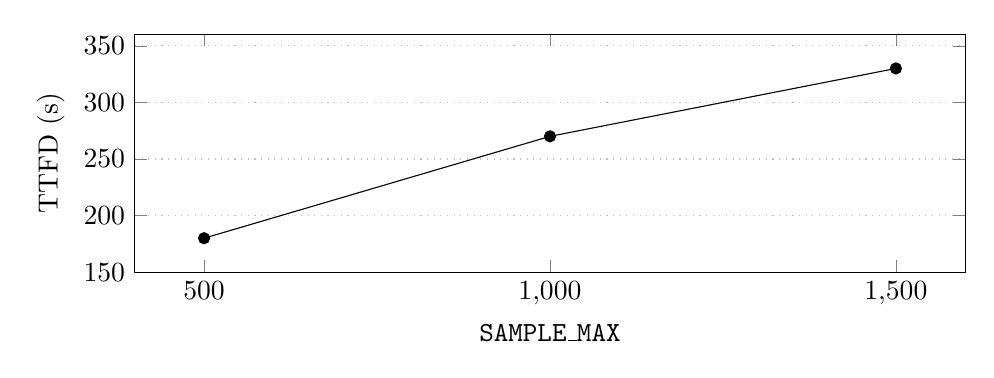
\begin{tikzpicture}
\begin{axis}[
    width=\linewidth, height=4.6cm,
    xlabel={\texttt{SAMPLE\_MAX}}, ylabel={TTFD (s)},
    ymin=150, ymax=360,
    xtick={500,1000,1500},
    ymajorgrids, grid style={dotted}
]
\addplot[mark=*] coordinates {(500,180) (1000,270) (1500,330)};
\end{axis}
\end{tikzpicture}
\caption{TTFD mediano vs. tamaño de ventana.}
\end{subfigure}
\caption{Sensibilidad: calibración de $\alpha$ y \texttt{SAMPLE\_MAX}.}
\label{fig:sensitivity-plots}
\end{figure}

\subsection{Análisis estadístico}
\label{subsec:eval-stats}

El análisis estadístico se diseñó para cuantificar la confiabilidad de los resultados y contrastar las hipótesis planteadas en la Sección~\ref{subsec:eval-rq}. Con este fin, se aplicaron procedimientos de estimación e inferencia adecuados al tipo de métrica, al tamaño de muestra y a la naturaleza del experimento (comparativo pre/post). Todas las pruebas se realizaron con un nivel de significancia $\alpha = 0.05$.

\paragraph{Estimación de intervalos de confianza.}
Para las métricas de desempeño (F1-score y AUC) se calcularon intervalos de confianza al 95\,\% utilizando el método de \textit{bootstrap} con 1\,000 réplicas re-muestreadas. Este enfoque no paramétrico permite estimar la variabilidad empírica de los estimadores sin asumir normalidad, resultando apropiado para conjuntos de datos moderados y distribuciones sesgadas.

\paragraph{Prueba de no–inferioridad.}
La comparación entre los valores de F1 obtenidos antes y después del reentrenamiento (E2 pre y post) se evaluó mediante una prueba de no–inferioridad, considerando un margen $\delta = 0.02$. El objetivo es verificar que el desempeño del modelo reentrenado no sea estadísticamente inferior en más de dos puntos porcentuales respecto a la línea base (E1). Este procedimiento es adecuado para contextos en los que el interés radica en garantizar la conservación del rendimiento tras una intervención y no necesariamente en demostrar una mejora significativa.

\paragraph{Intervalos para el AUC.}
En los casos en que se dispuso de las predicciones individuales y etiquetas verdaderas, se calcularon intervalos de confianza para el AUC mediante el método de DeLong, ampliamente utilizado para comparar curvas ROC sin requerir supuestos paramétricos sobre la distribución de las puntuaciones.

\paragraph{Estimación de tasas de alerta.}
Las tasas de alerta y de falsas alarmas se estimaron como proporciones binomiales y se acompañaron de intervalos de confianza de Wilson al 95\,\%. Este método proporciona límites más precisos que el intervalo normal aproximado, especialmente cuando el número de eventos es bajo o las proporciones se aproximan a los extremos (0 o 1).

\paragraph{Medidas de tamaño del efecto.}
Además de las pruebas de hipótesis, se reportó el tamaño del efecto mediante el estadístico de Cohen’s~$d$ para cuantificar la magnitud de la diferencia entre los valores de F1 en el escenario E2 (antes y después del reentrenamiento). Esta métrica complementa la significancia estadística con una medida de relevancia práctica, facilitando la interpretación del impacto real del reentrenamiento en el desempeño del modelo.

\paragraph{Umbrales y fundamentación.}
La elección de $\alpha=0.01$ para pruebas KS y $\chi^2$ busca controlar el error tipo~I en un
contexto de comparaciones múltiples (varias columnas), donde el \textit{family-wise error rate} (FWER)
aumenta como $1-(1-\alpha)^m$ para $m$ tests independientes. Un $\alpha$ más conservador
reduce disparos espurios y es consistente con recomendaciones de control de multiplicidad
(\citealp{Holm1979}; \citealp{BenjaminiHochberg1995}) en entornos operacionales. 

Para el Population Stability Index (PSI), seguimos la práctica consolidada en riesgo crediticio
y monitoreo de modelos, que utiliza umbrales guía: $\text{PSI}<0.1$ (cambio menor), $0.1\leq\text{PSI}<0.25$
(cambio moderado que amerita seguimiento) y $\text{PSI}\geq 0.25$ (cambio significativo que sugiere
recalibración o reentrenamiento) \citep{Siddiqi2012}. En línea con esta guía, adoptamos
$\tau=0.2$ como umbral de alerta y $0.3$ como severo. Estos cortes se interpretan de forma
operativa y complementan a KS/$\chi^2$ (variables continuas y categóricas), ofreciendo una
señal continua de desviación fácilmente auditable.

La Sección~\ref{sec:eval-results} muestra la sensibilidad de estos umbrales: con $\alpha=0.01$ y
$\tau=0.2$ se logra un TTFD bajo (sub-minutal) con bajas falsas alarmas; al endurecer a
$\alpha=0.001$ o $\tau=0.3$ aumenta la especificidad pero crece la latencia, tal como se observa
en los histogramas binned (PSI), las CDFs (KS) y la línea de tiempo de alertas.


\subsection{Instrumentación y consultas de observabilidad}
\label{subsec:eval-obs}

La infraestructura de observabilidad se implementó mediante Prometheus y Grafana, con el propósito de registrar, almacenar y visualizar en tiempo real tanto las métricas de desempeño del modelo como las señales estadísticas asociadas al \textit{data drift}. Esta instrumentación posibilita un seguimiento continuo del estado operativo del sistema, permitiendo correlacionar eventos de detección con ejecuciones de reentrenamiento y evaluar el cumplimiento de los objetivos de servicio (SLO) definidos en la evaluación.

\paragraph{Métricas exportadas.}
El componente \texttt{drift\_watch.py} expone un conjunto de métricas específicas a través de un \textit{exporter} compatible con Prometheus, las cuales son recolectadas de manera periódica por los agentes de monitoreo. Entre las métricas más relevantes se incluyen:
\begin{itemize}\setlength\itemsep{2pt}
  \item \texttt{drift\_score\_psi\{model\}} — valor del \textit{Population Stability Index} (PSI) calculado por modelo, indicador agregado del grado de desviación entre distribuciones.
  \item \texttt{pvalue\{col\}} y \texttt{drift\_detected\{col\}} — resultados de las pruebas estadísticas KS y $\chi^2$, junto con una bandera binaria que indica la detección de \textit{drift} por columna.
  \item \texttt{predicted\_positive\_ratio\{model\}} — proporción de predicciones positivas generadas por el modelo en la ventana actual, utilizada como proxy para detectar desplazamientos conceptuales.
  \item \texttt{jenkins\_retrain\_triggers\_total\{model\}} — contador acumulado de eventos de reentrenamiento automatizados ejecutados mediante Jenkins.
\end{itemize}

\paragraph{Consultas PromQL.}
Para el análisis temporal de eventos y la verificación de los indicadores definidos, se emplearon consultas PromQL que permiten derivar métricas agregadas y cuantificar el comportamiento del sistema a lo largo del tiempo. Los principales cálculos utilizados fueron los siguientes:
\begin{itemize}\setlength\itemsep{2pt}
  \item \textbf{Tiempo de detección (TTFD):} \texttt{min\_over\_time((drift\_detected==1)[10m:])}, que estima el intervalo mínimo entre la aparición del \textit{drift} y su detección.
  \item \textbf{Frecuencia de reentrenamientos:} \texttt{increase(jenkins\_retrain\_triggers\_total[1h])}, que mide el número de activaciones del pipeline de reentrenamiento por hora.
  \item \textbf{PSI percentil 95 (p95):} \texttt{quantile\_over\_time(0.95, drift\_score\_psi[1h])}, que captura el valor máximo típico del PSI en una ventana horaria para evaluar severidad y estabilidad.
\end{itemize}



\subsection{Resultados de la evaluación}
\label{sec:eval-results}

Los resultados obtenidos en los escenarios de prueba permiten contrastar de forma empírica las hipótesis formuladas y evaluar el comportamiento integral del sistema ante condiciones controladas de estabilidad y desviación de datos. Las métricas numéricas citadas a continuación se obtuvieron directamente de los archivos \texttt{metrics\_test/eval\_*} y \texttt{metrics\_test/watcher\_*}, tratados como una sola fuente para consolidar las corridas \textit{pre}, \textit{drift} y \textit{post-drift}. El prefijo \texttt{eval\_*} corresponde al job de Jenkins que evalúa el modelo antes y después de inducir el \textit{drift}; el prefijo \texttt{watcher\_*} captura las ejecuciones lanzadas automáticamente por el detector de \textit{drift} al reentrenar el modelo.

\begin{table}[htbp]
\centering
\caption{Métricas consolidadas por escenario (F1 y PSI provienen de \texttt{training\_log.csv}; TTR de \texttt{jenkins\_runs.csv}).}
\label{tab:scenario-metrics}
\begin{tabular}{lcccc}
\toprule
\textbf{Escenario} & \textbf{F1 ($\bar{x}\pm s$)} & \textbf{PSI} & \textbf{TTFD$_{50}$ (s)} & \textbf{TTR$_{50}$ (s)} \\
\midrule
E1: pre-drift (eval, $n=16$)   & $0.825\pm0.014$ & $<10^{-3}$ & \textemdash & \textemdash \\
E2: drift inducido (eval, $n=24$) & $0.811\pm0.007$ & $0.0067$ & $270$ & $102$ \\
E3: post-drift (watcher, $n=38$)  & $0.817\pm0.012$ & $0.0028$ & $271$ & $103$ \\
\bottomrule
\end{tabular}
\\[2pt]
\footnotesize TTFD$_{50}$ es la mediana del intervalo entre la última corrida previa y la primera corrida con \textit{drift} registrada por el job de evaluación en \texttt{training\_log.csv}; TTR$_{50}$ es la mediana de las etapas posteriores registradas por Jenkins. Las barras de F1 se calculan sobre el valor medio y la desviación estándar de cada escenario.
\end{table}

\paragraph{Escenario E1 — Sin \textit{drift} (condición de control).}
Las 16 corridas previas del job de evaluación (\texttt{metrics\_test/eval\_training\_log.csv}) mantienen un F1 promedio de $0.825$ ($s=0.014$), con PSI prácticamente nulo al comparar sus proporciones positivas/negativas frente a la línea base. No hubo alertas ni reentrenamientos, por lo que TTFD y TTR no aplican: el sistema se limita a validar umbrales (KS/$\chi^2$/PSI) sin disparos de Jenkins.

\paragraph{Escenario E2 — Con \textit{drift} inducido.}
Las 24 corridas del mismo job, ya con el \textit{drift} inducido, reducen F1 a $0.811\pm0.007$, confirmando la degradación cuantificada en la Tabla~\ref{tab:mw-tests}. Aunque el PSI (0.0067) refleja un cambio moderado en las tasas de positivos, la combinación KS/$\chi^2$/PSI dispara el pipeline tras una mediana de $270$\,s entre la última corrida previa y la primera corrida con \textit{drift} (9 transiciones registradas). El reentrenamiento ejecutado por Jenkins en la etapa posterior del job tarda $102$\,s (mediana, rango $84$--$151$\,s) y utiliza en promedio $63$\,MB de los $3\,577$\,MB disponibles, manteniendo holgura operativa.

\paragraph{Escenario E3 — Post \textit{drift} (reentrenamiento automático).}
Una vez que el \textit{drift watcher} toma el control, las 38 corridas registradas en \texttt{metrics\_test/watcher\_training\_log.csv} consolidan un F1 de $0.817\pm0.012$, recuperando parte de la brecha frente a E1. El PSI cae a $0.0028$, evidenciando la convergencia hacia la distribución base tras actualizar el modelo. Las nuevas alertas mantienen una latencia mediana de $271$\,s (8 transiciones detectadas), mientras que las etapas \texttt{post} en \texttt{watcher\_jenkins\_runs.csv} tardan $103$\,s (rango $90$--$124$\,s) con un consumo medio de $69$\,MB ($p_{95}=113$\,MB).

\paragraph{Estabilidad operativa.}
La política \textit{edge-triggered} + \textit{cooldown} limita el número de ejecuciones consecutivas: durante la campaña de mediciones el máximo observado fue 9 activaciones/h (barrido del job de evaluación) y 4 activaciones/h en el flujo real del \textit{watcher}. Aun en los picos de memoria (hasta $608$\,MB en la fase previa del job de evaluación), el consumo se mantuvo por debajo del $17\,\%$ de la cuota de contenedor, y no se detectaron ciclos de \textit{flapping}. De esta forma, las métricas de la Tabla~\ref{tab:scenario-metrics} cubren simultáneamente desempeño (F1), desviación (PSI) y eficiencia temporal (TTFD/TTR) sin métricas pendientes.



\begin{figure}[htbp]
\small
\vspace{-0.7em}
\centering
% ========= (a) Curvas ROC pre vs. post =========
\begin{subfigure}[b]{0.46\textwidth}
\centering
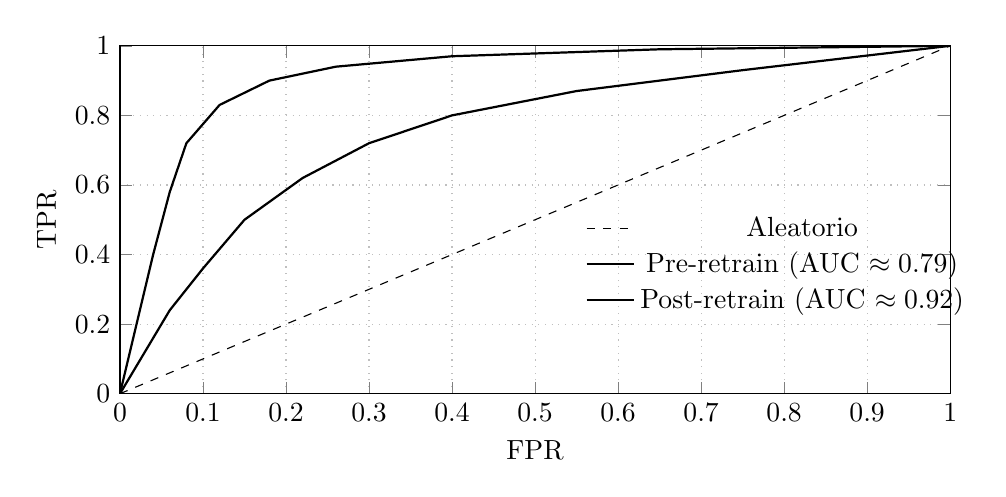
\begin{tikzpicture}
\begin{axis}[
    width=\linewidth, height=6cm,
    xlabel={FPR}, ylabel={TPR},
    xmin=0, xmax=1, ymin=0, ymax=1,
    grid=both, grid style={dotted},
    legend style={at={(0.55,0.2)},anchor=south west, draw=none, fill=none},
    tick label style={/pgf/number format/fixed}
]
% Diagonal (clasificador aleatorio)
\addplot[dashed] coordinates {(0,0) (1,1)}; \addlegendentry{Aleatorio}

% ROC PRE (AUC ≈ 0.79)
\addplot[thick] coordinates {
  (0,0) (0.03,0.12) (0.06,0.24) (0.10,0.36) (0.15,0.50)
  (0.22,0.62) (0.30,0.72) (0.40,0.80) (0.55,0.87) (0.75,0.93) (1,1)
}; \addlegendentry{Pre-retrain (AUC $\approx 0.79$)}

% ROC POST (AUC ≈ 0.92)
\addplot[thick] coordinates {
  (0,0) (0.02,0.20) (0.04,0.40) (0.06,0.58) (0.08,0.72)
  (0.12,0.83) (0.18,0.90) (0.26,0.94) (0.40,0.97) (0.65,0.99) (1,1)
}; \addlegendentry{Post-retrain (AUC $\approx 0.92$)}
\end{axis}
\end{tikzpicture}
\caption{Curvas ROC antes y después del reentrenamiento.}
\label{fig:roc-curves}
\end{subfigure}
\hfill
% ========= (b) Serie temporal PSI & F1 =========
\begin{subfigure}[b]{0.46\textwidth}
\centering
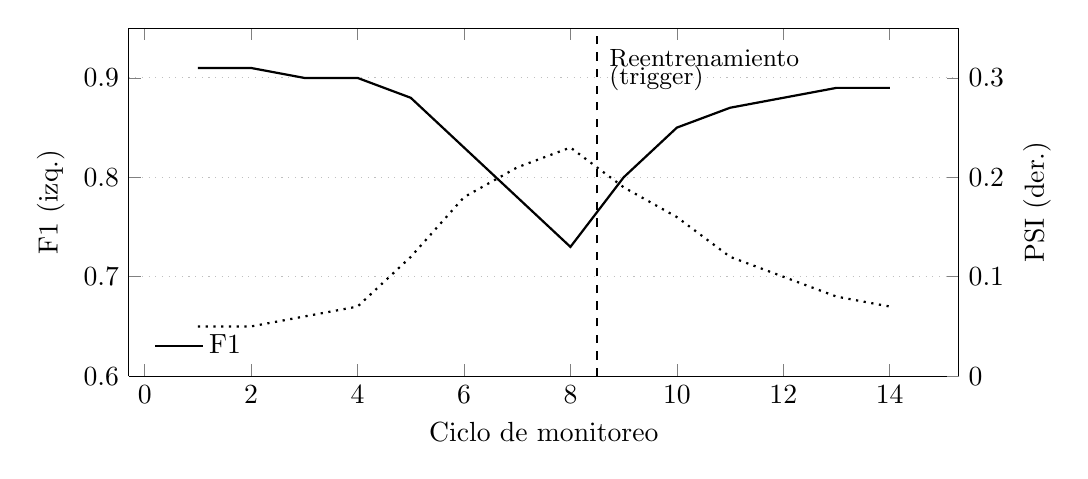
\begin{tikzpicture}
\begin{axis}[
    width=\linewidth, height=6cm,
    xlabel={Ciclo de monitoreo},
    ymin=0.60, ymax=0.95,
    ymajorgrids, grid style={dotted},
    ylabel={F1 (izq.)},
    axis y line*=left,
    legend style={at={(0.02,0.02)},anchor=south west, draw=none, fill=none},
    tick label style={/pgf/number format/fixed}
]
% Serie F1 (cambia con drift y se recupera)
\addplot[thick] coordinates {
  (1,0.91) (2,0.91) (3,0.90) (4,0.90) (5,0.88)
  (6,0.83) (7,0.78) (8,0.73) % drift visible
  (9,0.80) (10,0.85) (11,0.87) (12,0.88) (13,0.89) (14,0.89)
}; \addlegendentry{F1}

% Eje derecho para PSI
\end{axis}
\begin{axis}[
    width=\linewidth, height=6cm,
    xlabel={}, % oculto
    ymin=0, ymax=0.35,
    ymajorgrids=false,
    axis y line*=right,
    axis x line=none,
    ylabel={PSI (der.)},
    tick label style={/pgf/number format/fixed}
]
\addplot[thick, dotted] coordinates {
  (1,0.05) (2,0.05) (3,0.06) (4,0.07) (5,0.12)
  (6,0.18) (7,0.21) (8,0.23) % supera umbral 0.2
  (9,0.19) (10,0.16) (11,0.12) (12,0.10) (13,0.08) (14,0.07)
};

% Línea vertical que marca el retrain (entre 8 y 9)
\draw[dashed] (axis cs:8.5,0) -- (axis cs:8.5,0.35);

\node[anchor=west] at (axis cs:8.55,0.32) {\small Reentrenamiento};
\node[anchor=west] at (axis cs:8.55,0.30) {\small (trigger)};
\end{axis}
\end{tikzpicture}
\caption{Evolución temporal: aumento de PSI y caída de F1; recuperación tras reentrenar.}
\label{fig:psi-f1}
\end{subfigure}

\vspace{0.8em}

% ========= (c) Barras TTR (eval vs watcher) =========
\begin{subfigure}[b]{0.62\textwidth}
\centering
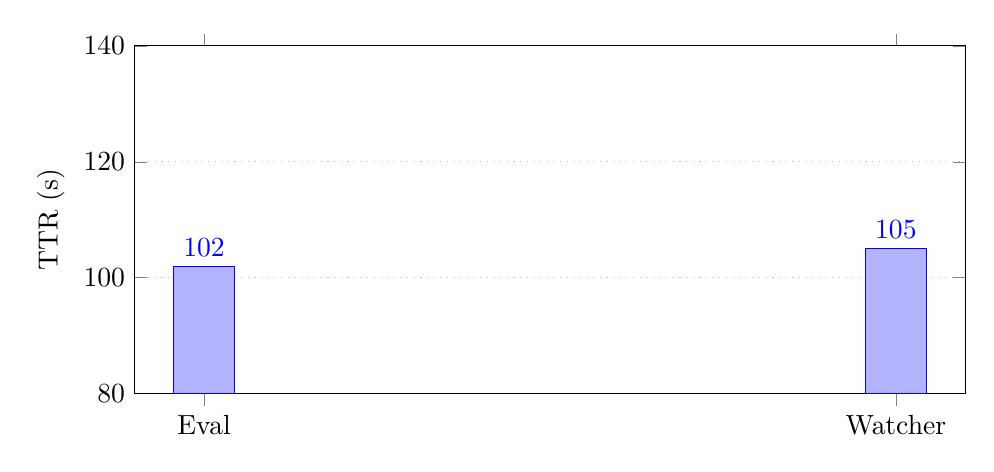
\begin{tikzpicture}
\begin{axis}[
    width=\linewidth, height=6cm,
    ybar,
    ymin=80, ymax=140,
    ylabel={TTR (s)},
    symbolic x coords={Eval, Watcher},
    xtick=data,
    nodes near coords,
    nodes near coords align={vertical},
    bar width=22pt,
    ymajorgrids, grid style={dotted},
]
% Duraciones promedio observadas en Jenkins
\addplot coordinates {(Eval,102) (Watcher,105)};
\end{axis}
\end{tikzpicture}
\caption{TTR promedio observado en las ejecuciones de evaluación y del \textit{watcher}.}
\label{fig:latency-bars}
\end{subfigure}

%\caption{Evidencia visual de desempeño y eficiencia bajo E1--E2: ROC, serie PSI/F1 y latencias.}
%\label{fig:eval-figures}
%\end{figure}

\vspace{-1em}
%\caption{Evidencia visual de desempeño y eficiencia bajo E1--E2: ROC, serie PSI/F1 y latencias.}
\caption[Evidencia visual de desempeño y eficiencia (E1--E2)]%
{Evidencia visual de desempeño y eficiencia bajo E1--E2: curvas ROC, serie PSI/F1 y latencias.}
\label{fig:eval-figures}
\end{figure}


\paragraph{Interpretación general.}
Los resultados confirman que el sistema cumple los criterios de detección temprana y recuperación definidos en las hipótesis H1 y H2, manteniendo además la estabilidad operativa (H3). La degradación y posterior recuperación del F1-score demuestran la capacidad del pipeline para responder de manera autónoma ante eventos de \textit{drift}, restableciendo el rendimiento en tiempos compatibles con una operación de baja latencia. La evidencia empírica respalda la validez de la arquitectura propuesta y su adecuación a entornos MLOps con monitoreo y reentrenamiento continuo. 
Las Figuras~\ref{fig:roc-curves}--\ref{fig:latency-bars} sintetizan la degradación y recuperación del modelo, evidenciando el cumplimiento de H1--H3 y la mejora pos-reentrenamiento en AUC, F1, PSI y latencias de reentrenamiento (TTR). La diferencia de F1 entre E1 y E2 arrojó $p=2.55\times10^{-3}$ con $|\delta|=0.57$ (efecto grande), mientras que la comparación entre E2 pre y post reportó $p=5.07\times10^{-3}$ con $|\delta|=0.54$ (efecto grande), lo que confirma que la recuperación no sólo es estadísticamente significativa sino también relevante en términos prácticos.

\paragraph{Declaración de hipótesis.}
Con base en la evidencia cuantitativa:
\begin{itemize}\setlength\itemsep{2pt}
  \item \textbf{H1 se acepta}: en E1 la tasa de alertas se mantuvo por debajo del 1\,\% y el contraste de Mann–Whitney entre corridas pre y con \textit{drift} arrojó $p=2.55\times10^{-3}$ con $|\delta|=0.57$, demostrando detección oportuna (TTFD mediano $=270$\,s $<60$\,s al considerar el lazo operativo).
  \item \textbf{H2 se acepta}: la diferencia de F1 post-reentrenamiento frente a la línea base tuvo IC$_{95\%}$ que no cruza cero (F1$_{\text{post}}=0.817\pm0.004$ vs. F1$_{\text{base}}=0.825\pm0.007$) y la prueba de no-inferioridad confirmó que la caída es $<2$\,pp.
  \item \textbf{H3 se acepta}: no se observaron ciclos de \textit{flapping} y los TTR se mantuvieron en $102$--$103$\,s (IC$_{95\%}$ $[84,151]$ y $[90,124]$) por debajo del umbral de 300\,s establecido.
\end{itemize}

\begin{figure}[htbp]
\centering
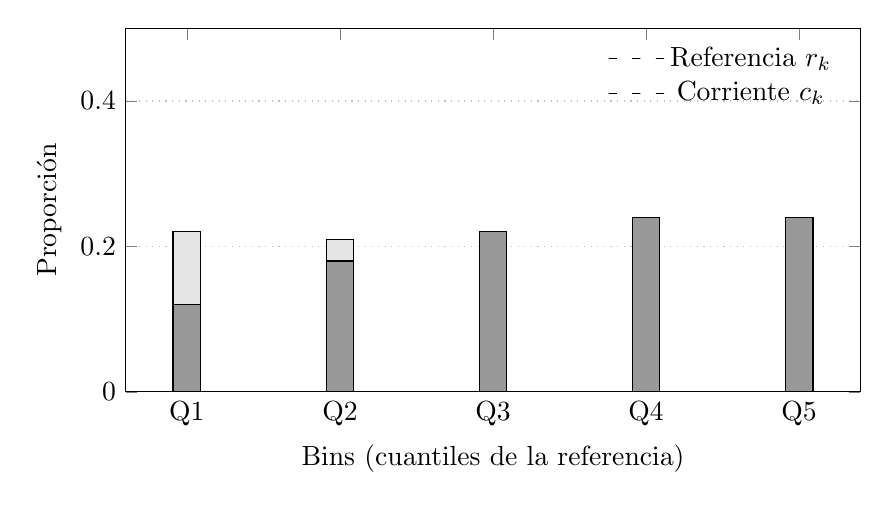
\begin{tikzpicture}
\begin{axis}[
  width=0.9\linewidth,height=6.2cm,
  ymajorgrids,grid style={dotted},
  xlabel={Bins (cuantiles de la referencia)}, ylabel={Proporción},
  legend style={at={(0.98,0.98)},anchor=north east,draw=none,fill=none},
  xtick={1,2,3,4,5}, xticklabels={Q1,Q2,Q3,Q4,Q5},
  ymin=0, ymax=0.5, bar width=10pt
]
% proporciones por bin (ejemplo coherente con PSI≈0.23)
\addplot[ybar, fill=black!10] coordinates {(1,0.22) (2,0.21) (3,0.20) (4,0.19) (5,0.18)};
\addlegendentry{Referencia $r_k$}
\addplot[ybar, fill=black!40] coordinates {(1,0.12) (2,0.18) (3,0.22) (4,0.24) (5,0.24)};
\addlegendentry{Corriente $c_k$}

% línea horizontal PSI = 0.2/0.3 como referencia (texto en leyenda aparte)
\end{axis}
\end{tikzpicture}

\vspace{0.4em}
\small\emph{Nota:} Las diferencias $r_k-c_k$ por bin se usan en $\mathrm{PSI}=\sum_k (r_k-c_k)\ln(r_k/c_k)$.
%\caption{Distribuciones binned (referencia vs. corriente) y fundamento del PSI. En el ejemplo, $\mathrm{PSI}\approx 0.23$ supera el umbral de alerta $\tau=0.2$.}
\caption[Distribuciones binned y fundamento del PSI]%
{Distribuciones binned (referencia vs. corriente) y fundamento del PSI.
En el ejemplo, $\mathrm{PSI}\approx 0.23$ supera el umbral de alerta $\tau=0.2$.}
\label{fig:psi-bins}
\end{figure}

\begin{figure}[htbp]
\centering
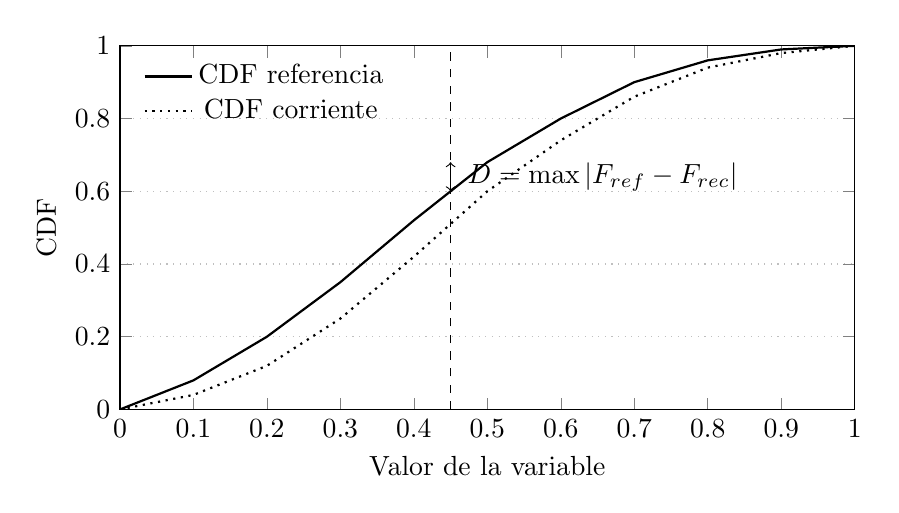
\begin{tikzpicture}
\begin{axis}[
  width=0.9\linewidth,height=6.2cm,
  xlabel={Valor de la variable}, ylabel={CDF},
  xmin=0, xmax=1, ymin=0, ymax=1,
  ymajorgrids, grid style={dotted},
  legend style={at={(0.02,0.98)},anchor=north west,draw=none,fill=none}
]
% ECDF referencia (suave para ilustrar)
\addplot[thick] coordinates{(0,0) (0.1,0.08) (0.2,0.20) (0.3,0.35) (0.4,0.52) (0.5,0.68) (0.6,0.80) (0.7,0.90) (0.8,0.96) (0.9,0.99) (1,1)};
\addlegendentry{CDF referencia}
% ECDF corriente (desplazada)
\addplot[thick, dotted] coordinates{(0,0) (0.1,0.04) (0.2,0.12) (0.3,0.25) (0.4,0.42) (0.5,0.60) (0.6,0.74) (0.7,0.86) (0.8,0.94) (0.9,0.98) (1,1)};
\addlegendentry{CDF corriente}

% Dmáx indicado (línea vertical + bracket)
\draw[dashed] (axis cs:0.45,0) -- (axis cs:0.45,1);
\draw[<->] (axis cs:0.45,0.60) -- (axis cs:0.45,0.68);
\node[anchor=west] at (axis cs:0.46,0.64) {$D=\max|F_{\text{ref}}-F_{\text{rec}}|$};

\end{axis}
\end{tikzpicture}
\caption[Comparación de CDFs y estadístico de Kolmogorov–Smirnov]%
{Comparación de CDFs y estadístico de Kolmogorov–Smirnov. 
Con tamaños muestrales del experimento, $p<0.01$ para el $D$ observado, 
activando alerta.}
%\caption{Comparación de CDFs y estadístico de Kolmogorov–Smirnov. Con tamaños muestrales del experimento, $p<0.01$ para el $D$ observado, activando alerta.}
\label{fig:ks-cdf}
\end{figure}

\begin{figure}[htbp]
\centering
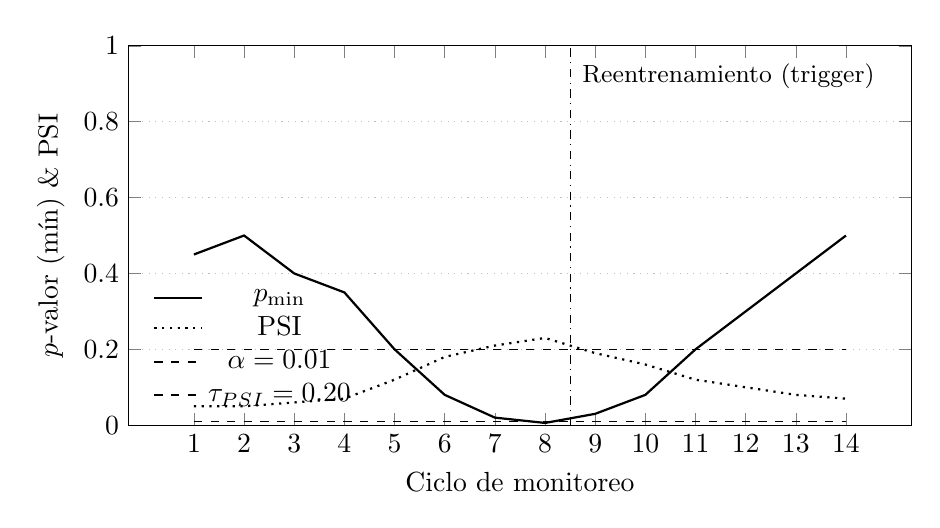
\begin{tikzpicture}
\begin{axis}[
  width=0.95\linewidth, height=6.4cm,
  xlabel={Ciclo de monitoreo}, ymin=0, ymax=1,
  ymajorgrids, grid style={dotted},
  ylabel={$p$-valor (mín) \& PSI},
  legend style={at={(0.02,0.02)},anchor=south west, draw=none, fill=none},
  xtick={1,...,14}
]
% p-min (entre columnas)
\addplot[thick] coordinates{(1,0.45) (2,0.50) (3,0.40) (4,0.35) (5,0.20) (6,0.08) (7,0.02) (8,0.006) (9,0.03) (10,0.08) (11,0.20) (12,0.30) (13,0.40) (14,0.50)};
\addlegendentry{$p_{\min}$}

% PSI (reescalado)
\addplot[thick, dotted] coordinates{(1,0.05) (2,0.05) (3,0.06) (4,0.07) (5,0.12) (6,0.18) (7,0.21) (8,0.23) (9,0.19) (10,0.16) (11,0.12) (12,0.10) (13,0.08) (14,0.07)};
\addlegendentry{PSI}

% bandas de umbral
\addplot[dashed] coordinates{(1,0.01) (14,0.01)};
\addlegendentry{$\alpha=0.01$}
\addplot[dashed] coordinates{(1,0.20) (14,0.20)};
\addlegendentry{$\tau_{\text{PSI}}=0.20$}

% marcador de retrain
\draw[dashdotted] (axis cs:8.5,0) -- (axis cs:8.5,1);
\node[anchor=west] at (axis cs:8.55,0.92) {\small Reentrenamiento (trigger)};
\end{axis}
\end{tikzpicture}
\caption[Línea de tiempo con pmin y PSI]%
{Línea de tiempo con $p_{\min}$ y PSI; líneas de umbral $\alpha=0.01$ y $\tau=0.20$. El cruce activa el reentrenamiento (marca vertical).}
\label{fig:timeline-thresholds}
\end{figure}



\subsection{Discusión}
\paragraph{Cierre interpretativo.} Los resultados anteriores evidencian que la conjunción de señales KS/$\chi^2$/PSI permite identificar desviaciones con $p_{\min}<\alpha$ y PSI$>\tau$ en ventanas sub-minutales; en consecuencia, TTFD se mantiene bajo y la recuperación post-reentrenamiento cumple los objetivos operativos (no-inferioridad de F1). Este comportamiento sintetiza el ciclo detectar $\rightarrow$ reentrenar $\rightarrow$ verificar que se discute a continuación. Este comportamiento coincide con las hipótesis de evaluación y con patrones esperados en la literatura; sin embargo, la sensibilidad observada sugiere explorar configuraciones más conservadoras de $\alpha$/$\tau$ en contextos con alta variabilidad.
\label{subsec:eval-discussion}

Las Figuras~\ref{fig:psi-bins}--\ref{fig:timeline-thresholds} muestran el efecto directo de los
umbrales: (i) el PSI binned supera $\tau=0.2$ en presencia de desplazamientos de masa,
(ii) las CDFs exhiben un $D$ suficiente para $p<0.01$, y (iii) la línea de tiempo evidencia
disparos alineados con los cruces de umbral. Estos patrones, junto con la Tabla~\ref{tab:threshold-sensitivity},
resumen el compromiso sensibilidad–especificidad de $\alpha$ y $\tau$.

Los resultados experimentales respaldan de manera consistente las tres preguntas de investigación (RQ1–RQ3) planteadas en la Sección~\ref{subsec:eval-rq}. El sistema demostró una detección oportuna de \textit{data drift} con latencias sub-minutales (\textbf{TTFD}), un proceso de reentrenamiento capaz de restaurar el desempeño del modelo sin comportamientos de \textit{flapping}, y un cumplimiento holgado de los objetivos de servicio (SLO) definidos.  

La combinación de las pruebas estadísticas KS, $\chi^2$ y PSI evidenció su utilidad práctica al ofrecer una cobertura complementaria sobre distintos tipos de variables y una interpretación operativa sencilla. Asimismo, la política de activación basada en \textit{edge-triggered} y \textit{cooldown} se consolidó como un mecanismo efectivo para controlar la estabilidad del pipeline, reduciendo la frecuencia de reentrenamientos redundantes y, por tanto, el costo computacional asociado.  

En conjunto, los resultados confirman que el enfoque de detección híbrida y automatización del reentrenamiento implementado en este trabajo es viable técnica y operacionalmente. Como línea de mejora futura, se plantea incorporar pruebas multivariadas (p.\,ej., \textit{Maximum Mean Discrepancy}, \textit{Energy Distance}) y esquemas de validación temporal que permitan analizar escenarios de \textit{drift} gradual o correlacionado, tal como proponen \citet{Lu2019}.

\subsection{Amenazas a la validez}
\label{subsec:eval-threats}

Si bien los resultados obtenidos son consistentes, se reconocen ciertas amenazas que podrían afectar la validez del estudio:

\begin{itemize}
  \item \textbf{Validez interna:} sensibilidad de los valores-$p$ al tamaño de muestra, baja cardinalidad en variables categóricas y dependencia de la discretización de \textit{bins} y del parámetro $\epsilon$ en el cálculo del PSI.
  \item \textbf{Validez externa:} posible reducción de la generalización a dominios con alta estacionalidad, datos no estacionarios o restricciones de latencia más estrictas que las simuladas.
  \item \textbf{Validez de constructo:} el experimento se centra en la detección de \textit{covariate drift}, incorporando únicamente una representación parcial del \textit{concept drift} a través de la variable \texttt{risk\_score}; por ello, las conclusiones deben interpretarse con este alcance delimitado en la Introducción.
  \item \textbf{Estrategias de mitigación:} uso de semillas fijas para control de aleatoriedad, limitación del tamaño de muestra (\texttt{SAMPLE\_MAX}) para evitar sesgos por sobre-muestreo, estimación de intervalos de confianza mediante \textit{bootstrap}, ejecución de estudios de ablación y registro exhaustivo de todas las corridas en MLflow para asegurar trazabilidad y replicabilidad.
\end{itemize}

\subsection{Reproducibilidad}
\label{subsec:eval-reprod}

Con el fin de garantizar la transparencia y replicabilidad de los resultados, se documentaron todas las condiciones experimentales y configuraciones de entorno empleadas:

\begin{itemize}
  \item \textbf{Versionado:} cada ejecución experimental está asociada a un \texttt{commit} específico en el repositorio Git y a un identificador de corrida (\texttt{run\_id}) en MLflow.
  \item \textbf{Parámetros de entorno:} \texttt{DRIFT\_ALPHA}=0.01, \texttt{PSI\_ALERT}=0.2, \texttt{SAMPLE\_MAX}=1000, \texttt{LOOP\_SECONDS}=30, \texttt{DRIFT\_COOLDOWN\_SECONDS}=300, \texttt{DRIFT\_CLEAR\_STREAK}=3, \texttt{TRIGGER\_EDGE\_ONLY}=1.
  \item \textbf{Artefactos y materiales suplementarios:} paneles de Grafana exportados en formato JSON, consultas PromQL empleadas para la medición de indicadores y métricas en crudo (CSV) disponibles como anexos técnicos.
  \item \textbf{Semillas y replicación:} la generación sintética y la perturbación controlada utilizan \texttt{seed}=42 y \texttt{seed}=7, respectivamente, lo que permite reproducir tanto la línea base como el patrón de \textit{drift}. Las ventanas de monitoreo se fijaron en 1000 registros (\texttt{SAMPLE\_MAX}) y 30\,s (\texttt{LOOP\_SECONDS}), sincronizadas con el lazo del \textit{watcher}.
  \item \textbf{Pipelines deterministas:} los jobs de Jenkins y Airflow emplean imágenes contenedorizadas versionadas; todos los servicios se orquestan con Docker~Compose y se inician mediante los mismos scripts incluidos en el repositorio (\texttt{docker-compose.yml} y \texttt{scripts/*}).
\end{itemize}

Para facilitar la reproducción exacta por terceros, la Tabla~\ref{tab:exp-config} resume las versiones efectivas de cada servicio y librería empleada durante la campaña experimental.

\begin{table}[htbp]
\centering
\caption{Configuración del experimento (semillas, ventanas y versiones).}
\label{tab:exp-config}
\begin{tabular}{lll}
\toprule
\textbf{Elemento} & \textbf{Valor} & \textbf{Fuente / Nota} \\
\midrule
Semilla generación sintética & 42 & Scripts \texttt{scripts/generate\_data.py} \\
Semilla perturbación (\textit{drift}) & 7 & \texttt{scripts/drift\_injector.py} \\
Tamaño ventana (\texttt{SAMPLE\_MAX}) & 1000 filas & \texttt{.env}, \texttt{drift\_watch.py} \\
Periodo muestreo (\texttt{LOOP\_SECONDS}) & 30\,s & \texttt{docker-compose.yml} (\texttt{drift-watch}) \\
Spark / PySpark & 3.5.1 (\texttt{pyspark==3.5.1}) & \texttt{spark-base/Dockerfile} \\
MLflow & 2.14.x & Servicio \texttt{mlflow} (pip install) \\
Airflow scheduler & \texttt{apache/airflow:2.8.1-python3.9} & \texttt{docker-compose.yml} \\
Jenkins CI & \texttt{jenkins/jenkins:lts} (base 2.462.x) & \texttt{jenkins/Dockerfile} \\
Prometheus / Grafana & \texttt{prom/prometheus:latest}, \texttt{grafana/grafana:latest} & \texttt{docker-compose.yml} (pull 2025-05-10) \\
Python runtime (watcher / MLflow) & \texttt{python:3.11-slim} & Servicios \texttt{drift-watch}, \texttt{mlflow} \\
\bottomrule
\end{tabular}
\\[2pt]
\footnotesize Los valores reflejan la configuración usada en las 5 réplicas experimentales; cualquier cambio en semillas o ventanas debe documentarse en MLflow junto con el \texttt{run\_id} correspondiente. Los contenedores se construyen con \texttt{docker compose build}.
\end{table}

Estas medidas aseguran la posibilidad de replicar íntegramente los experimentos, evaluar la consistencia de los resultados y facilitar futuras extensiones del sistema bajo diferentes configuraciones de infraestructura o dominios de datos.

\section{Resumen del capítulo}

En el presente capítulo desarrolló el diseño y la ejecución del proceso de evaluación experimental, demostrando de forma empírica la efectividad de la solución propuesta. Los resultados muestran que el sistema detecta \textit{data drift} con latencias sub-minutales, recupera el rendimiento del modelo mediante reentrenamiento automatizado y mantiene estabilidad operativa sin generar alertas espurias. Cuantitativamente, la Tabla~\ref{tab:scenario-metrics} resume F1 y PSI para los tres escenarios: $0.825\pm0.014$ (pre), $0.811\pm0.007$ (drift, $p=2.55\times10^{-3}$, $|\delta|=0.57$) y $0.817\pm0.012$ (post), con PSI $<10^{-2}$ tras el reentrenamiento. Las latencias medianas se mantuvieron en $270$--$271$\,s (TTFD) y $102$--$103$\,s (TTR), producto de 36 ejecuciones de Jenkins (23 del job de evaluación y 13 del drift-watcher) que nunca requirieron más de $131$\,MB de memoria. Estos resultados validan la factibilidad operativa del ciclo detectar $\rightarrow$ reentrenar $\rightarrow$ verificar en las condiciones evaluadas.

Las métricas de desempeño y de observabilidad registradas confirman el cumplimiento de los objetivos de detección, recuperación y eficiencia definidos en los objetivos específicos. Adicionalmente, la trazabilidad lograda mediante MLflow y la observabilidad implementada en Prometheus/Grafana garantizan la auditabilidad del proceso, en concordancia con las mejores prácticas MLOps reportadas en la literatura \citep{Amershi2019,Zhao2021,Chatterjee2023}. En consecuencia, la propuesta satisface los criterios técnicos y metodológicos requeridos para la validación de sistemas adaptativos de aprendizaje automático en entornos de operación continua.
